\subsection{Frequency Response Matching\label{sec:ch6:freqresponse}}

\subsubsection{Synthesis Task}
The first example is based on Ref.~\cite{Grimbleby1995a}. Here we wish to synthesize circuits that match the following frequency response:
\begin{align}
\abs{F(j \omega)} = \sqrt{\frac{2 \pi}{10 \omega}}
\end{align}

\noindent over the frequency range:
\begin{align*}
0.2 \leq \frac{\omega}{2\pi} \leq 5
\end{align*}

\noindent with 500 logarithmically spaced evaluation points.
Since we have a desired magnitude response, not an explicit transfer function, traditional design methods cannot accommodate this synthesis task \cite{Grimbleby1995a}.

We will consider two sets of simple bounds on the coefficients of the resistors and capacitors:
\begin{align*}
\text{(set 1)} &\qquad \gls{resistance}\in[10^{-2}, 10^{0}]\ \Omega, \quad \gls{capacitance} \in [10^{-2}, 10^{0}] \text{ F} \\
\text{(set 2)} &\qquad R\in[10^{-2}, 10^{5}]\ \Omega, \quad C \in [10^{-10}, 10^{0}] \text{ F}
\end{align*}

\noindent and there are no additional general constraints.
The residual function is the pointwise decibel error in Eqn.~(\ref{eq:ch6:rk:1}).

\subsubsection{Circuit Structure Space\label{sec:ch6:mm:css}}

The desired circuit structure space is ``all topologies that have up to 6 impedance subcircuits and a required connection to the ground.''
Such a space is captured by:
\begin{subequations}
\label{eq:ch6:lib2}
\begin{align}
C &= \{ \xcolor{I}, \xcolor{O}, \xcolor{G}, \xcolor{Z}, \xcolor{N3}, \xcolor{N4}, \xcolor{N5}, \xcolor{N6}, \xcolor{N7}, \xcolor{N8}, \xcolor{N9} \} \\
P &=        \left[ 1\ 1\ 1\ 2\ 3\ 4\ 5\ 6\ 7\ 8\ 9 \right] \\
R_{\min} &= \left[ 1\ 1\ 1\ 1\ 0\ 0\ 0\ 0\ 0\ 0\ 0 \right] \\
R_{\max} &= \left[ 1\ 1\ 1\ 6\ 5\ 3\ 3\ 2\ 1\ 1\ 1 \right]
\end{align}
\end{subequations}

\noindent and includes all the NSCs from Sec.~\ref{sec:ch6:primitive}.
Only nine different orders of voltage nodes are used, as any higher-order nodes would not produce feasible topologies.
The specific values of $R_{\max}$ are the maximum number of replicates needed to still capture all possible feasible subcatalogs with respect to Eqn.~(\ref{eq:ch6:subcatalog:feas}).
The subcircuits for generating practical circuits will be series connections between $\{\xcolor{R}, \xcolor{C}\}$ components to replicate the elements available in Ref.~\cite{Grimbleby1995a}.
The primitive circuit library then has 393 unique graphs, and these graphs are expanded to 104,235 unique practical circuit graphs (see Table~\ref{tb:ch6:mm1:computational}).

\begin{table}[ht]
\centering
\caption{Computational cost of \nameref{sec:ch6:freqresponse} example.\label{tb:ch6:mm1:computational}}
\begin{tabular}{rrrr}
\hline \hline
                                    & Step                   & $t$ (s) & $N$ \\
\hline
\multirow{3}{*}{Circuit generation} & Primitive circuits     & 78 &  393 \\
                                    & Practical circuits     & 131  & 104,235  \\
                                    & Transfer functions     & 14,379  & 43,249   \\
 \arrayrulecolor{gray}\hline\arrayrulecolor{black}
 \multirow{2}{*}{Evaluation}        & Ref.~\cite{Grimbleby1995a}, set 1 & 29,303  & 43,249    \\
 & Ref.~\cite{Grimbleby1995a}, set 2 & 28,739  & 43,249    \\
\hline \hline
\end{tabular}
\end{table}

This synthesis task will utilize the template circuit in Fig.~\ref{fig:ch6:template:magnitude}.
Of the 104,235 practical circuit graphs, 43,249 were found to have unique transfer functions.
This difference is attributed to cases where two circuits that have the same transfer function but different colored graph representations.
For example, in some practical circuits, components do not show up in the transfer function (due to a functional short between the input and output nodes).
In these cases, the lower complexity circuit is always kept.
With the desired circuit library, we can now perform the sizing task to determine which circuits better satisfy the requirements of the synthesis task.

\subsubsection{Results}

\begin{figure*}[t]
\centering
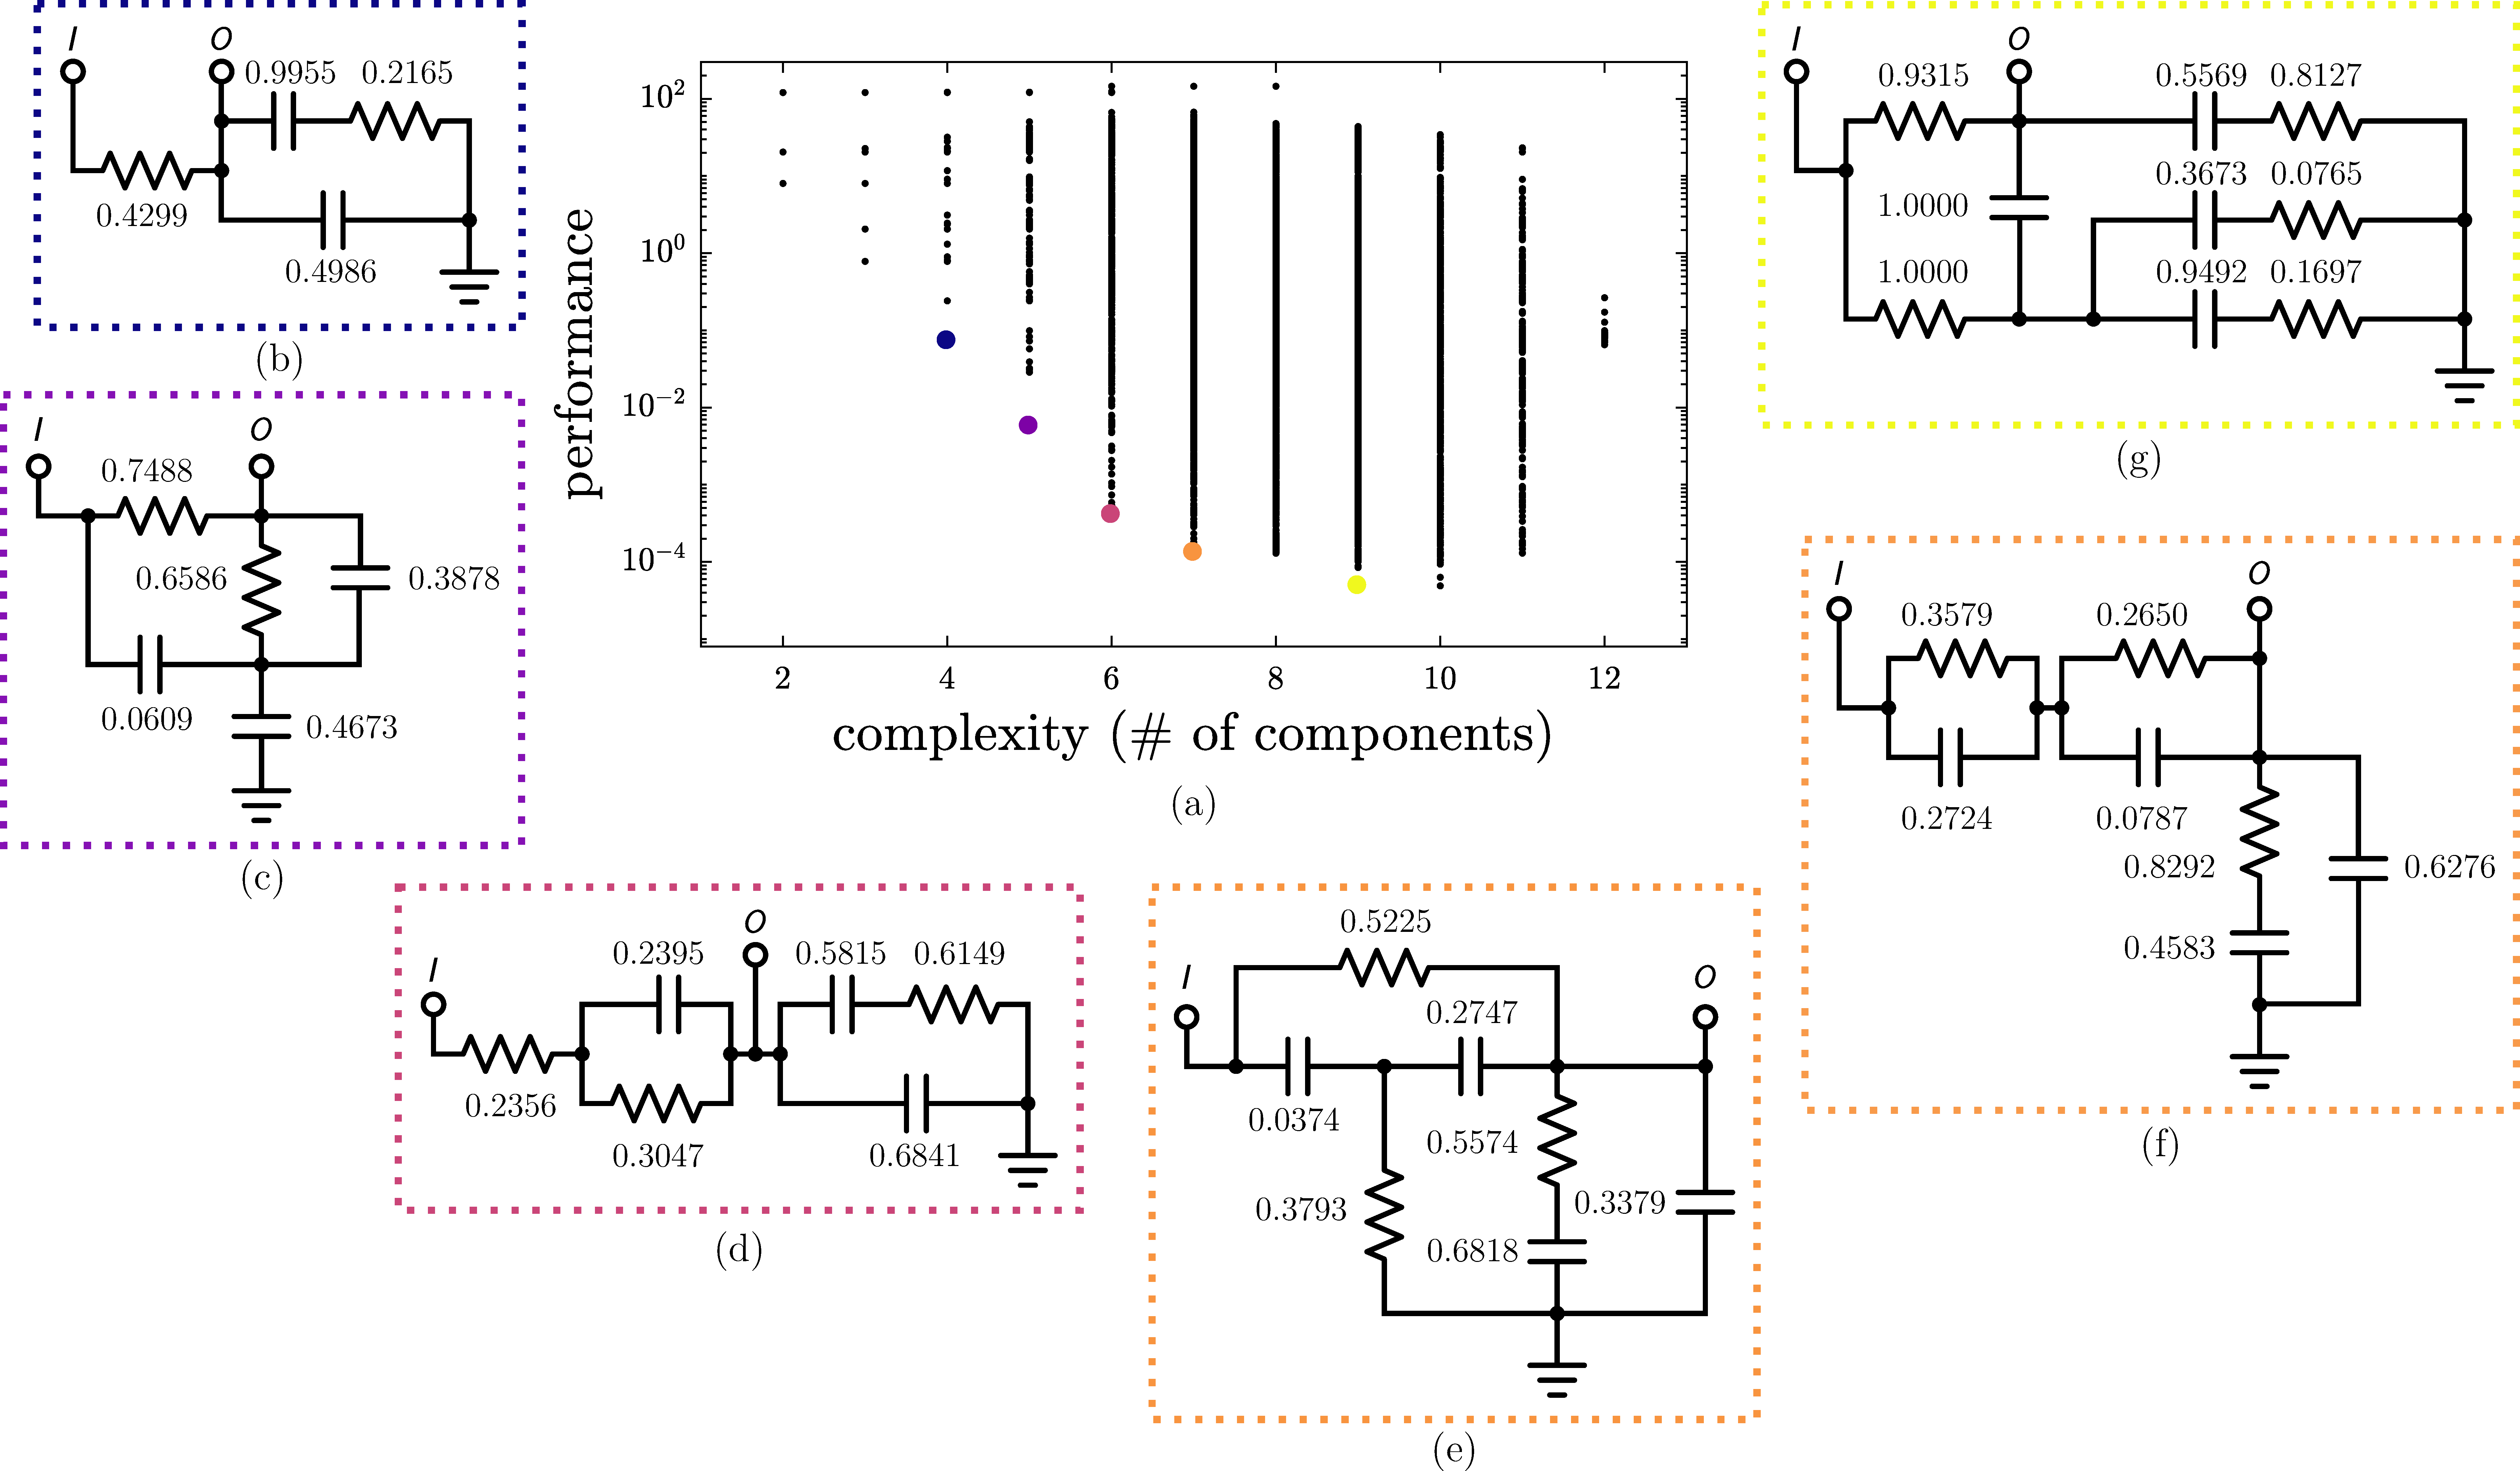
\includegraphics[width=\textwidth]{../ch6/figures/reduced/r_ex1_set1}
\caption[Performance vs. complexity for \nameref{sec:ch6:freqresponse} example using set 1 along with select Pareto optimal circuits.]{Performance vs. complexity (\# of components) for \nameref{sec:ch6:freqresponse} example using set 1 along with select Pareto optimal circuits (units are $\Omega$ and F).\label{fig:ch6:ex1:set1}}
\end{figure*}

The results for set 1 are summarized in Fig.~\ref{fig:ch6:ex1:set1}a where the performance for every circuit is shown, stratified by the complexity (or number of components).   
Select Pareto-optimal (performance cannot be improved without an increase in complexity) circuits are also shown in Figs.~\ref{fig:ch6:ex1:set1}a--g.
The desired magnitude response can be seen in Fig.~\ref{fig:mm1_magnitude} along with $\abs{G}$ for select circuits in Fig.~\ref{fig:ch6:ex1:set1}.

\begin{figure}
\centering
\begin{subfigure}[t]{0.5\textwidth}
\centering
% 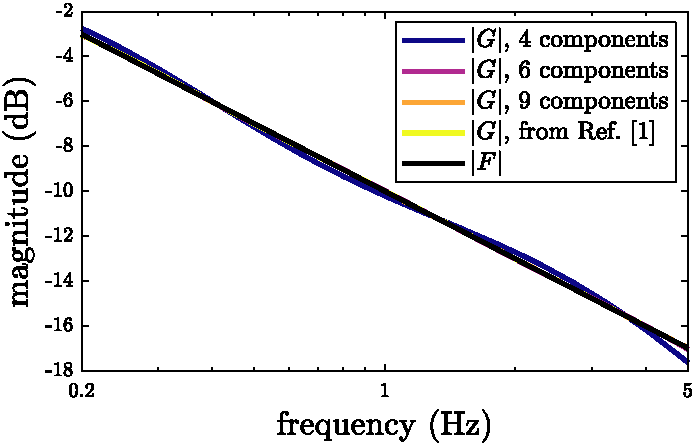
\includegraphics[width=\textwidth]{../ch6/figures/mm1_magnitude.pdf}
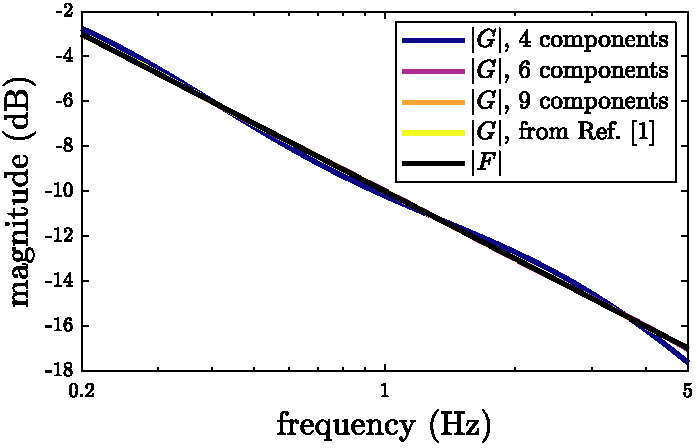
\includegraphics[width=\textwidth]{../ch6/figures/reduced/r_mm1_magnitude}
\caption{Both desired and circuit magnitude response.\label{fig:mm1_magnitude}}
\end{subfigure}%
\begin{subfigure}[t]{0.5\textwidth}
\centering
% 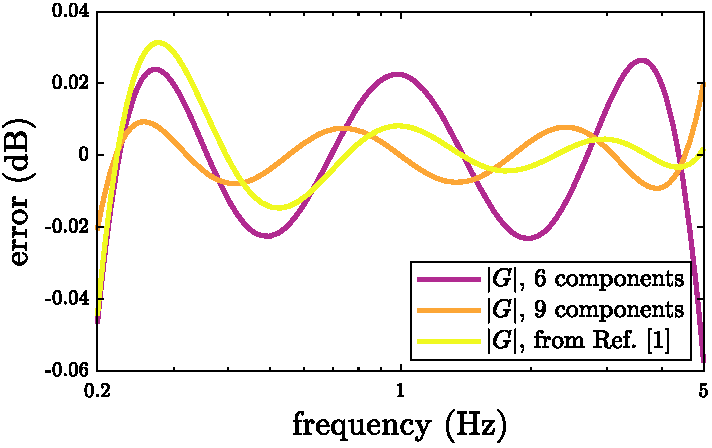
\includegraphics[width=\textwidth]{../ch6/figures/mm1_errors}
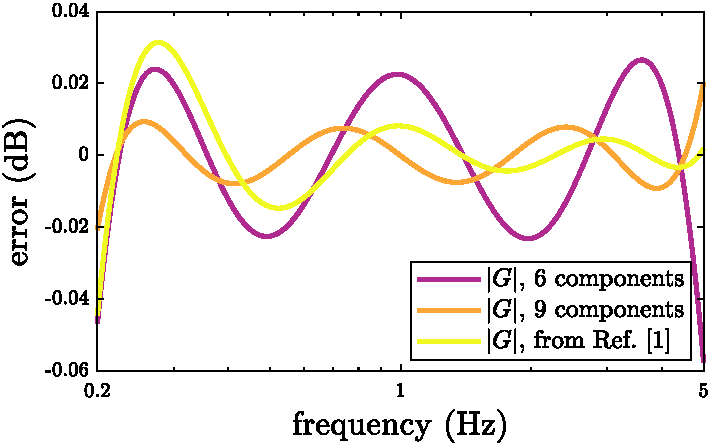
\includegraphics[width=\textwidth]{../ch6/figures/reduced/r_mm1_errors}
\caption{Errors.\label{fig:mm1_errors}}
\end{subfigure}%

\caption[Magnitude and errors over the desired frequency range using select circuits.]{Magnitude and errors over the desired frequency range using select circuits from Fig.~\ref{fig:ch6:ex1:set1}.\label{fig:mm1_magerrors}}

\end{figure}

% new paragraph
In fact, the included circuits are not unique Pareto-optimal circuits. 
For complexity levels of $\{4,5,6,7,9\}$, there are $\{5,22,57,200,2\}$ different circuits that produce the same level of performance.
This is due to each having nearly identical transfer functions using different circuit topologies.
For a specified number of poles and zeros, there is a lower bound on the performance (nonzero in this task) defined by a transfer function where the coefficients are tuned directly (sometimes called complex-curve fitting \cite{Levy1959a}).
Therefore, a set of circuits perform as well as possible under the pole/zero limitations defined by the circuit structure space and complexity level.
For example, consider the circuit in Fig.~\ref{fig:ch6:ex1:set1}b where $G$ contains 2 zeros and 3 poles, and produces a performance level of $7.3 \times 10^{-2}$. If we instead designed the polynomial coefficients directly, the lower bound on the performance is $2.9 \times 10^{-2}$; which is similar to the synthesized circuit but smaller.
See Table~\ref{tb:ch6:mm1:besttransfer} for this comparison at additional complexity levels and note the trend in the optimal orders of \gls{nz} and \gls{np}.

\begin{table}[ht]
\centering
\caption[Performance comparison between best and arbitrary circuit transfer functions.]{Performance level comparison between best circuit transfer function and best arbitrary transfer function for various complexity levels.\label{tb:ch6:mm1:besttransfer}}
\begin{tabular}{rrrrr}
\hline \hline
& & & \multicolumn{2}{c}{Performance} \\
$n_c$ & $n_z^{\glsfoo[noindex]{optimal}}$ & $n_p^*$ & Best circuit $G$ & Best $G$ \\
\hline
4 & 2 & 3 & $7.3\times10^{-2}$ & $2.9\times10^{-2}$ \\
5 & 3 & 3 & $5.7\times10^{-3}$ & $3.4\times10^{-3}$ \\
6 & 3 & 4 & $4.1\times10^{-4}$ & $4.0\times10^{-4}$ \\
7 & 4 & 4 & $1.3\times10^{-4}$ & $4.8\times10^{-5}$ \\
8 & 4 & 5 & $1.3\times10^{-4}$ & $5.6\times10^{-6}$ \\
9 & 5 & 5 & $4.8\times10^{-5}$ & $6.6\times10^{-7}$  \\
\hline \hline
\end{tabular}
\end{table}

% new paragraph
In a similar manner as set 1, the results for set 2 are summarized in
Fig.~\ref{fig:mm1_results_set2}.
In this set of results, an interesting pattern emerges, namely more discrete groupings of the performance levels and similarly valued groups are shared between different complexity levels.
With increased flexibility in the values of the passive component's coefficients, transfer functions with similar properties (e.g.,~the same order for $n_z$ and $n_p$) are attracted to similar performance levels during sizing.
This is further illustrated in Fig.~\ref{fig:mm1_cumpercent} where the performance is plotted by cumulative percentage of circuits that have at least the given performance level.
For set 1 we see little pattern in the performance curve but with set 2, we see more discrete performance levels.
In this figure we also see more circuits achieving a specified level of performance with the increased variable ranges in set 2 (i.e.,~the curve for set 2 is always below set 1).
In addition, many more circuits achieve the best performance level, but there is only a minor reduction of the objective compared to circuits sized using set 1.

\begin{figure}
\centering
% 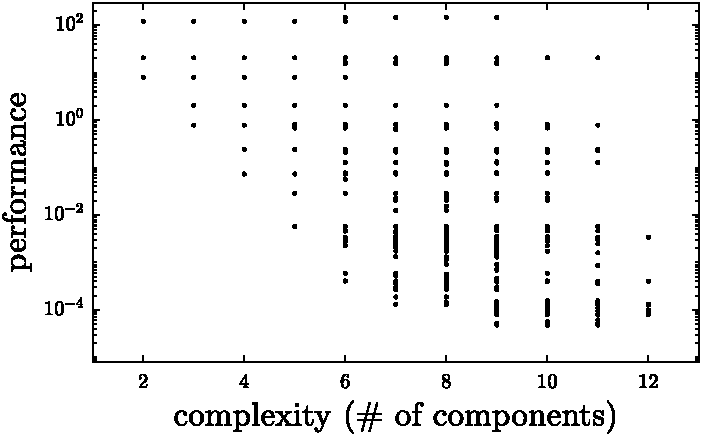
\includegraphics[width=0.9\columnwidth]{../ch6/figures/template1_lib5_CR_RESULTS_SET2}
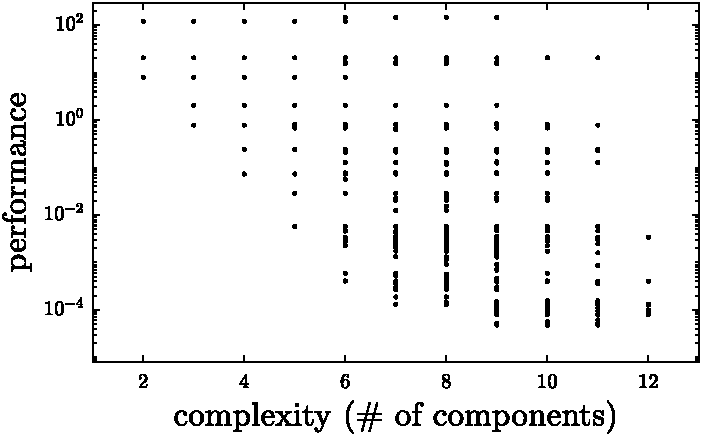
\includegraphics[width=0.5\textwidth]{../ch6/figures/reduced/r_template1_lib5_CR_RESULTS_SET2}
\caption[Performance vs. complexity for \nameref{sec:ch6:freqresponse} example using set 2.]{Performance vs. complexity (\# of components) for \nameref{sec:ch6:freqresponse} example using set 2.\label{fig:mm1_results_set2}}
\end{figure}

\begin{figure}[t]
\centering

\includegraphics[width=0.2\columnwidth]{../ch6/figures/template1_lib5_CR_RESULTS_Legend_FINAL.pdf}

\vspace{0.05in}

\begin{subfigure}[b]{0.3\columnwidth}
\centering
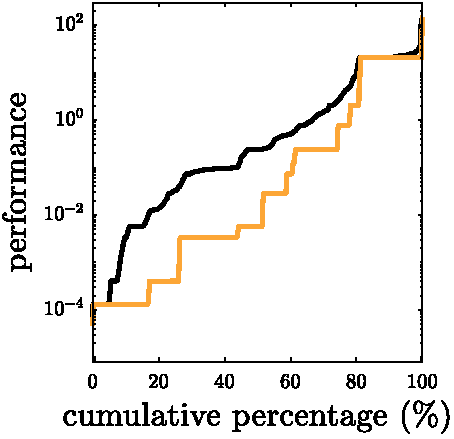
\includegraphics[width=\textwidth]{../ch6/figures/template1_lib5_CR_RESULTS}
\caption{All circuits.}
\end{subfigure}%
\begin{subfigure}[b]{0.3\columnwidth}
\centering
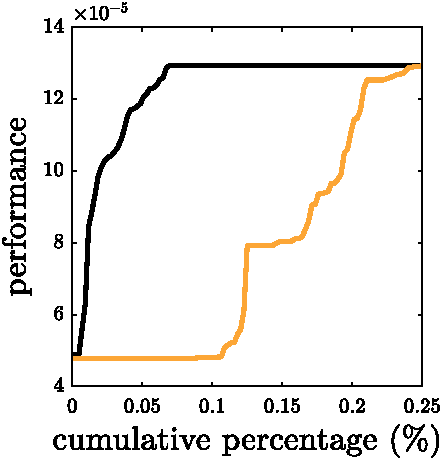
\includegraphics[width=\textwidth]{../ch6/figures/template1_lib5_CR_RESULTS_2}
\caption{Best circuits.}
\end{subfigure}%
\caption{Performance vs. cumulative percentage for \nameref{sec:ch6:freqresponse} example.\label{fig:mm1_cumpercent}}
\end{figure}

% new paragraph
A circuit of particular interest is the one found in Fig.~\ref{fig:ch6:ex1:set1}e, as it has the same topology as the circuit reported in Ref.~\cite{Grimbleby1995a}.
Since the topology and sizing tasks were performed simultaneously using an evolutionary approach in Ref.~\cite{Grimbleby1995a}, it could have been challenging to converge to the local optimum (something gradient-based methods do well).
However, it is extremely impressive that the synthesized circuit in Ref.~\cite{Grimbleby1995a} was close to the Pareto frontier (same topology, slightly worse performance level at $3.0 \times 10^{-4}$ with the error visualized in Fig.~\ref{fig:mm1_errors}).

% new paragraph
While the circuit in Fig.~\ref{fig:ch6:ex1:set1}g has the best performance level (under the enumerated circuit structure space), it would be up to the designer to decide if the increase in complexity is worth the performance improvement.
Having a large number of options provides the designer with additional flexibility when selecting a final circuit.